% !TeX document-id = {58dd56a7-a545-4332-9f31-aa9515ad78e0}
%%%%%%%%%%%%%%%%%%%%%%%%%%%%%%%%%%%%%%%%%
% The Legrand Orange Book
% LaTeX Template
% Version 2.4 (26/09/2018)
%
% This template was downloaded from:
% http://www.LaTeXTemplates.com
%
% Original author:
% Mathias Legrand (legrand.mathias@gmail.com) with modifications by:
% Vel (vel@latextemplates.com)
%
% License:
% CC BY-NC-SA 3.0 (http://creativecommons.org/licenses/by-nc-sa/3.0/)
%
% Compiling this template:
% This template uses biber for its bibliography and makeindex for its index.
% When you first open the template, compile it from the command line with the
% commands below to make sure your LaTeX distribution is configured correctly:
%
% 1) pdflatex main
% 2) makeindex main.idx -s StyleInd.ist
% 3) biber main
% 4) pdflatex main x 2
%
% After this, when you wish to update the bibliography/index use the appropriate
% command above and make sure to compile with pdflatex several times
% afterwards to propagate your changes to the document.
%
% This template also uses a number of packages which may need to be
% updated to the newest versions for the template to compile. It is strongly
% recommended you update your LaTeX distribution if you have any
% compilation errors.
%
% Important note:
% Chapter heading images should have a 2:1 width:height ratio,
% e.g. 920px width and 460px height.
%
%%%%%%%%%%%%%%%%%%%%%%%%%%%%%%%%%%%%%%%%%

%----------------------------------------------------------------------------------------
%	PACKAGES AND OTHER DOCUMENT CONFIGURATIONS
%----------------------------------------------------------------------------------------

% !BIB program = biber
% !TeX TXS-program:compile = txs:///pdflatex/[--shell-escape]

\documentclass[11pt,fleqn]{book} % Default font size and left-justified equations

%%%%%%%%%%%%%%%%%%%%%%%%%%%%%%%%%%%%%%%%%
% The Legrand Orange Book
% Structural Definitions File
% Version 2.1 (26/09/2018)
%
% Original author:
% Mathias Legrand (legrand.mathias@gmail.com) with modifications by:
% Vel (vel@latextemplates.com)
%
% This file was downloaded from:
% http://www.LaTeXTemplates.com
%
% License:
% CC BY-NC-SA 3.0 (http://creativecommons.org/licenses/by-nc-sa/3.0/)
%
%%%%%%%%%%%%%%%%%%%%%%%%%%%%%%%%%%%%%%%%%

%----------------------------------------------------------------------------------------
%	VARIOUS REQUIRED PACKAGES AND CONFIGURATIONS
%----------------------------------------------------------------------------------------

\usepackage{graphicx} % Required for including pictures
\graphicspath{{assets/}} % Specifies the directory where pictures are stored

\usepackage{lipsum} % Inserts dummy text

\usepackage{tikz} % Required for drawing custom shapes

\usepackage[english]{babel} % English language/hyphenation

\usepackage{enumitem} % Customize lists
\setlist{nolistsep} % Reduce spacing between bullet points and numbered lists

\usepackage{booktabs} % Required for nicer horizontal rules in tables

\usepackage{xcolor} % Required for specifying colors by name
\definecolor{ocre}{RGB}{22,57,123} % Define the orange color used for highlighting throughout the book

%----------------------------------------------------------------------------------------
%	MARGINS
%----------------------------------------------------------------------------------------

\usepackage{geometry} % Required for adjusting page dimensions and margins

\geometry{
	paper=a4paper, % Paper size, change to letterpaper for US letter size
	top=3cm, % Top margin
	bottom=3cm, % Bottom margin
	left=3cm, % Left margin
	right=3cm, % Right margin
	headheight=14pt, % Header height
	footskip=1.4cm, % Space from the bottom margin to the baseline of the footer
	headsep=10pt, % Space from the top margin to the baseline of the header
	%showframe, % Uncomment to show how the type block is set on the page
}

%----------------------------------------------------------------------------------------
%	FONTS
%----------------------------------------------------------------------------------------

\usepackage{avant} % Use the Avantgarde font for headings
%\usepackage{times} % Use the Times font for headings
%\usepackage{helvet}
%\usepackage{mathptmx} % Use the Adobe Times Roman as the default text font together with math symbols from the Sym­bol, Chancery and Com­puter Modern fonts

\usepackage{microtype} % Slightly tweak font spacing for aesthetics
\usepackage[utf8]{inputenc} % Required for including letters with accents
\usepackage[T1]{fontenc} % Use 8-bit encoding that has 256 glyphs
\renewcommand{\familydefault}{cmss}

%----------------------------------------------------------------------------------------
%	BIBLIOGRAPHY AND INDEX
%----------------------------------------------------------------------------------------

\usepackage[style=numeric,citestyle=numeric,sorting=nyt,sortcites=true,autopunct=true,babel=hyphen,hyperref=true,abbreviate=false,backref=true,backend=biber]{biblatex}
\addbibresource{bibliography.bib} % BibTeX bibliography file
\defbibheading{bibempty}{}

\usepackage{calc} % For simpler calculation - used for spacing the index letter headings correctly
\usepackage{makeidx} % Required to make an index
\makeindex % Tells LaTeX to create the files required for indexing

%----------------------------------------------------------------------------------------
%	MAIN TABLE OF CONTENTS
%----------------------------------------------------------------------------------------

\usepackage{titletoc} % Required for manipulating the table of contents

\contentsmargin{0cm} % Removes the default margin

% Part text styling (this is mostly taken care of in the PART HEADINGS section of this file)
\titlecontents{part}
	[0cm] % Left indentation
	{\addvspace{20pt}\bfseries} % Spacing and font options for parts
	{}
	{}
	{}

% Chapter text styling
\titlecontents{chapter}
	[1.25cm] % Left indentation
	{\addvspace{12pt}\large\sffamily\bfseries} % Spacing and font options for chapters
	{\color{ocre!60}\contentslabel[\Large\thecontentslabel]{1.25cm}\color{ocre}} % Formatting of numbered sections of this type
	{\color{ocre}} % Formatting of numberless sections of this type
	{\color{ocre!60}\normalsize\;\titlerule*[.5pc]{.}\;\thecontentspage} % Formatting of the filler to the right of the heading and the page number

% Section text styling
\titlecontents{section}
	[1.25cm] % Left indentation
	{\addvspace{3pt}\sffamily\bfseries} % Spacing and font options for sections
	{\contentslabel[\thecontentslabel]{1.25cm}} % Formatting of numbered sections of this type
	{} % Formatting of numberless sections of this type
	{\hfill\color{black}\thecontentspage} % Formatting of the filler to the right of the heading and the page number

% Subsection text styling
\titlecontents{subsection}
	[1.25cm] % Left indentation
	{\addvspace{1pt}\sffamily\small} % Spacing and font options for subsections
	{\contentslabel[\thecontentslabel]{1.25cm}} % Formatting of numbered sections of this type
	{} % Formatting of numberless sections of this type
	{\ \titlerule*[.5pc]{.}\;\thecontentspage} % Formatting of the filler to the right of the heading and the page number

% Figure text styling
\titlecontents{figure}
	[1.25cm] % Left indentation
	{\addvspace{1pt}\sffamily\small} % Spacing and font options for figures
	{\thecontentslabel\hspace*{1em}} % Formatting of numbered sections of this type
	{} % Formatting of numberless sections of this type
	{\ \titlerule*[.5pc]{.}\;\thecontentspage} % Formatting of the filler to the right of the heading and the page number

% Table text styling
\titlecontents{table}
	[1.25cm] % Left indentation
	{\addvspace{1pt}\sffamily\small} % Spacing and font options for tables
	{\thecontentslabel\hspace*{1em}} % Formatting of numbered sections of this type
	{} % Formatting of numberless sections of this type
	{\ \titlerule*[.5pc]{.}\;\thecontentspage} % Formatting of the filler to the right of the heading and the page number

%----------------------------------------------------------------------------------------
%	MINI TABLE OF CONTENTS IN PART HEADS
%----------------------------------------------------------------------------------------

% Chapter text styling
\titlecontents{lchapter}
	[0em] % Left indentation
	{\addvspace{15pt}\large\sffamily\bfseries} % Spacing and font options for chapters
	{\color{ocre}\contentslabel[\Large\thecontentslabel]{1.25cm}\color{ocre}} % Chapter number
	{}
	{\color{ocre}\normalsize\sffamily\bfseries\;\titlerule*[.5pc]{.}\;\thecontentspage} % Page number

% Section text styling
\titlecontents{lsection}
	[0em] % Left indentation
	{\sffamily\small} % Spacing and font options for sections
	{\contentslabel[\thecontentslabel]{1.25cm}} % Section number
	{}
	{}

% Subsection text styling (note these aren't shown by default, display them by searchings this file for tocdepth and reading the commented text)
\titlecontents{lsubsection}
	[.5em] % Left indentation
	{\sffamily\footnotesize} % Spacing and font options for subsections
	{\contentslabel[\thecontentslabel]{1.25cm}}
	{}
	{}

%----------------------------------------------------------------------------------------
%	HEADERS AND FOOTERS
%----------------------------------------------------------------------------------------

\usepackage{fancyhdr} % Required for header and footer configuration

\pagestyle{fancy} % Enable the custom headers and footers

\renewcommand{\chaptermark}[1]{\markboth{\sffamily\normalsize\bfseries\chaptername\ \thechapter.\ #1}{}} % Styling for the current chapter in the header
\renewcommand{\sectionmark}[1]{\markright{\sffamily\normalsize\thesection\hspace{5pt}#1}{}} % Styling for the current section in the header

\fancyhf{} % Clear default headers and footers
\fancyhead[LE,RO]{\sffamily\normalsize\thepage} % Styling for the page number in the header
\fancyhead[LO]{\rightmark} % Print the nearest section name on the left side of odd pages
\fancyhead[RE]{\leftmark} % Print the current chapter name on the right side of even pages
%\fancyfoot[C]{\thepage} % Uncomment to include a footer

\renewcommand{\headrulewidth}{0.5pt} % Thickness of the rule under the header

\fancypagestyle{plain}{% Style for when a plain pagestyle is specified
	\fancyhead{}\renewcommand{\headrulewidth}{0pt}%
}

% Removes the header from odd empty pages at the end of chapters
\makeatletter
\renewcommand{\cleardoublepage}{
\clearpage\ifodd\c@page\else
\hbox{}
\vspace*{\fill}
\thispagestyle{empty}
\newpage
\fi}

%----------------------------------------------------------------------------------------
%	THEOREM STYLES
%----------------------------------------------------------------------------------------

\usepackage{amsmath,amsfonts,amssymb,amsthm} % For math equations, theorems, symbols, etc

\newcommand{\intoo}[2]{\mathopen{]}#1\,;#2\mathclose{[}}
\newcommand{\ud}{\mathop{\mathrm{{}d}}\mathopen{}}
\newcommand{\intff}[2]{\mathopen{[}#1\,;#2\mathclose{]}}
\renewcommand{\qedsymbol}{$\blacksquare$}
\newtheorem{notation}{Notation}[chapter]

% Boxed/framed environments
\newtheoremstyle{ocrenumbox}% Theorem style name
{0pt}% Space above
{0pt}% Space below
{\normalfont}% Body font
{}% Indent amount
{\small\bf\sffamily\color{ocre}}% Theorem head font
{\;}% Punctuation after theorem head
{0.25em}% Space after theorem head
{\small\sffamily\color{ocre}\thmname{#1}\nobreakspace\thmnumber{\@ifnotempty{#1}{}\@upn{#2}}% Theorem text (e.g. Theorem 2.1)
\thmnote{\nobreakspace\the\thm@notefont\sffamily\bfseries\color{black}---\nobreakspace#3.}} % Optional theorem note

\newtheoremstyle{blacknumex}% Theorem style name
{5pt}% Space above
{5pt}% Space below
{\normalfont}% Body font
{} % Indent amount
{\small\bf\sffamily}% Theorem head font
{\;}% Punctuation after theorem head
{0.25em}% Space after theorem head
{\small\sffamily{\tiny\ensuremath{\blacksquare}}\nobreakspace\thmname{#1}\nobreakspace\thmnumber{\@ifnotempty{#1}{}\@upn{#2}}% Theorem text (e.g. Theorem 2.1)
\thmnote{\nobreakspace\the\thm@notefont\sffamily\bfseries---\nobreakspace#3.}}% Optional theorem note

\newtheoremstyle{blacknumbox} % Theorem style name
{0pt}% Space above
{0pt}% Space below
{\normalfont}% Body font
{}% Indent amount
{\small\bf\sffamily}% Theorem head font
{\;}% Punctuation after theorem head
{0.25em}% Space after theorem head
{\small\sffamily\thmname{#1}\nobreakspace\thmnumber{\@ifnotempty{#1}{}\@upn{#2}}% Theorem text (e.g. Theorem 2.1)
\thmnote{\nobreakspace\the\thm@notefont\sffamily\bfseries---\nobreakspace#3.}}% Optional theorem note

% Non-boxed/non-framed environments
\newtheoremstyle{ocrenum}% Theorem style name
{5pt}% Space above
{5pt}% Space below
{\normalfont}% Body font
{}% Indent amount
{\small\bf\sffamily\color{ocre}}% Theorem head font
{\;}% Punctuation after theorem head
{0.25em}% Space after theorem head
{\small\sffamily\color{ocre}\thmname{#1}\nobreakspace\thmnumber{\@ifnotempty{#1}{}\@upn{#2}}% Theorem text (e.g. Theorem 2.1)
\thmnote{\nobreakspace\the\thm@notefont\sffamily\bfseries\color{black}---\nobreakspace#3.}} % Optional theorem note
\makeatother

% Defines the theorem text style for each type of theorem to one of the three styles above
\newcounter{dummy}
\numberwithin{dummy}{section}
\theoremstyle{ocrenumbox}
\newtheorem{theoremeT}[dummy]{Theorem}
\newtheorem{problem}{Problem}[chapter]
\newtheorem{exerciseT}{Exercise}[chapter]
\theoremstyle{blacknumex}
\newtheorem{exampleT}{Example}[chapter]
\theoremstyle{blacknumbox}
\newtheorem{vocabulary}{Vocabulary}[chapter]
\newtheorem{definitionT}{Definition}[section]
\newtheorem{corollaryT}[dummy]{Corollary}
\theoremstyle{ocrenum}
\newtheorem{proposition}[dummy]{Proposition}

% Library function description
\theoremstyle{ocrenumbox}
\newtheorem*{libfT}{Library}

%----------------------------------------------------------------------------------------
%	DEFINITION OF COLORED BOXES
%----------------------------------------------------------------------------------------

\RequirePackage[framemethod=default]{mdframed} % Required for creating the theorem, definition, exercise and corollary boxes

% Theorem box
\newmdenv[skipabove=7pt,
skipbelow=7pt,
backgroundcolor=black!5,
linecolor=ocre,
innerleftmargin=5pt,
innerrightmargin=5pt,
innertopmargin=5pt,
leftmargin=0cm,
rightmargin=0cm,
innerbottommargin=5pt]{tBox}

% Exercise box
\newmdenv[skipabove=7pt,
skipbelow=7pt,
rightline=false,
leftline=true,
topline=false,
bottomline=false,
backgroundcolor=ocre!10,
linecolor=ocre,
innerleftmargin=5pt,
innerrightmargin=5pt,
innertopmargin=5pt,
innerbottommargin=5pt,
leftmargin=0cm,
rightmargin=0cm,
linewidth=4pt]{eBox}

% Definition box
\newmdenv[skipabove=7pt,
skipbelow=7pt,
rightline=false,
leftline=true,
topline=false,
bottomline=false,
linecolor=ocre,
innerleftmargin=5pt,
innerrightmargin=5pt,
innertopmargin=0pt,
leftmargin=0cm,
rightmargin=0cm,
linewidth=4pt,
innerbottommargin=0pt]{dBox}

% Corollary box
\newmdenv[skipabove=7pt,
skipbelow=7pt,
rightline=false,
leftline=true,
topline=false,
bottomline=false,
linecolor=gray,
backgroundcolor=black!5,
innerleftmargin=5pt,
innerrightmargin=5pt,
innertopmargin=5pt,
leftmargin=0cm,
rightmargin=0cm,
linewidth=4pt,
innerbottommargin=5pt]{cBox}

% Creates an environment for each type of theorem and assigns it a theorem text style from the "Theorem Styles" section above and a colored box from above
\newenvironment{theorem}{\begin{tBox}\begin{theoremeT}}{\end{theoremeT}\end{tBox}}
\newenvironment{exercise}{\begin{eBox}\begin{exerciseT}}{\hfill{\color{ocre}\tiny\ensuremath{\blacktriangleleft}}\end{exerciseT}\end{eBox}}
\newenvironment{definition}{\begin{dBox}\begin{definitionT}}{\end{definitionT}\end{dBox}}
\newenvironment{example}{\begin{exampleT}}{\hfill{\tiny\ensuremath{\blacktriangleleft}}\end{exampleT}}
\newenvironment{corollary}{\begin{cBox}\begin{corollaryT}}{\end{corollaryT}\end{cBox}}

\newenvironment{libf}{\begin{tBox}\begin{libfT}}{\end{libfT}\end{tBox}}

%----------------------------------------------------------------------------------------
%	REMARK ENVIRONMENT
%----------------------------------------------------------------------------------------

\newenvironment{remark}{\par\vspace{10pt}\small % Vertical white space above the remark and smaller font size
\begin{list}{}{
\leftmargin=35pt % Indentation on the left
\rightmargin=25pt}\item\ignorespaces % Indentation on the right
\makebox[-2.5pt]{\begin{tikzpicture}[overlay]
\node[draw=ocre!60,line width=1pt,circle,fill=ocre!25,font=\sffamily\bfseries,inner sep=2pt,outer sep=0pt] at (-15pt,0pt){\textcolor{ocre}{$\bigstar$}};\end{tikzpicture}} % Orange R in a circle
\advance\baselineskip -1pt}{\end{list}\vskip5pt} % Tighter line spacing and white space after remark

%----------------------------------------------------------------------------------------
%	SECTION NUMBERING IN THE MARGIN
%----------------------------------------------------------------------------------------

\makeatletter
\renewcommand{\@seccntformat}[1]{\llap{\textcolor{ocre}{\csname the#1\endcsname}\hspace{1em}}}
\renewcommand{\section}{\@startsection{section}{1}{\z@}
{-4ex \@plus -1ex \@minus -.4ex}
{1ex \@plus.2ex }
{\normalfont\large\sffamily\bfseries}}
\renewcommand{\subsection}{\@startsection {subsection}{2}{\z@}
{-3ex \@plus -0.1ex \@minus -.4ex}
{0.5ex \@plus.2ex }
{\normalfont\sffamily\bfseries}}
\renewcommand{\subsubsection}{\@startsection {subsubsection}{3}{\z@}
{-2ex \@plus -0.1ex \@minus -.2ex}
{.2ex \@plus.2ex }
{\normalfont\small\sffamily\bfseries}}
\renewcommand\paragraph{\@startsection{paragraph}{4}{\z@}
{-2ex \@plus-.2ex \@minus .2ex}
{.1ex}
{\normalfont\small\sffamily\bfseries}}

%----------------------------------------------------------------------------------------
%	PART HEADINGS
%----------------------------------------------------------------------------------------

% Numbered part in the table of contents
\newcommand{\@mypartnumtocformat}[2]{%
	\setlength\fboxsep{0pt}%
	\noindent\colorbox{ocre!20}{\strut\parbox[c][.7cm]{\ecart}{\color{ocre!70}\Large\sffamily\bfseries\centering#1}}\hskip\esp\colorbox{ocre!40}{\strut\parbox[c][.7cm]{\linewidth-\ecart-\esp}{\Large\sffamily\centering#2}}%
}

% Unnumbered part in the table of contents
\newcommand{\@myparttocformat}[1]{%
	\setlength\fboxsep{0pt}%
	\noindent\colorbox{ocre!40}{\strut\parbox[c][.7cm]{\linewidth}{\Large\sffamily\centering#1}}%
}

\newlength\esp
\setlength\esp{4pt}
\newlength\ecart
\setlength\ecart{1.2cm-\esp}
\newcommand{\thepartimage}{}%
\newcommand{\partimage}[1]{\renewcommand{\thepartimage}{#1}}%
\def\@part[#1]#2{%
\ifnum \c@secnumdepth >-2\relax%
\refstepcounter{part}%
\addcontentsline{toc}{part}{\texorpdfstring{\protect\@mypartnumtocformat{\thepart}{#1}}{\partname~\thepart\ ---\ #1}}
\else%
\addcontentsline{toc}{part}{\texorpdfstring{\protect\@myparttocformat{#1}}{#1}}%
\fi%
\startcontents%
\markboth{}{}%
{\thispagestyle{empty}%
\begin{tikzpicture}[remember picture,overlay]%
\node at (current page.north west){\begin{tikzpicture}[remember picture,overlay]%
\fill[ocre!20](0cm,0cm) rectangle (\paperwidth,-\paperheight);
\node[anchor=north] at (4cm,-3.25cm){\color{ocre!40}\fontsize{220}{100}\sffamily\bfseries\thepart};
\node[anchor=south east] at (\paperwidth-1cm,-\paperheight+1cm){\parbox[t][][t]{8.5cm}{
\printcontents{l}{0}{\setcounter{tocdepth}{1}}% The depth to which the Part mini table of contents displays headings; 0 for chapters only, 1 for chapters and sections and 2 for chapters, sections and subsections
}};
\node[anchor=north east] at (\paperwidth-1.5cm,-3.25cm){\parbox[t][][t]{15cm}{\strut\raggedleft\color{white}\fontsize{30}{30}\sffamily\bfseries#2}};
\end{tikzpicture}};
\end{tikzpicture}}%
\@endpart}
\def\@spart#1{%
\startcontents%
\phantomsection
{\thispagestyle{empty}%
\begin{tikzpicture}[remember picture,overlay]%
\node at (current page.north west){\begin{tikzpicture}[remember picture,overlay]%
\fill[ocre!20](0cm,0cm) rectangle (\paperwidth,-\paperheight);
\node[anchor=north east] at (\paperwidth-1.5cm,-3.25cm){\parbox[t][][t]{15cm}{\strut\raggedleft\color{white}\fontsize{30}{30}\sffamily\bfseries#1}};
\end{tikzpicture}};
\end{tikzpicture}}
\addcontentsline{toc}{part}{\texorpdfstring{%
\setlength\fboxsep{0pt}%
\noindent\protect\colorbox{ocre!40}{\strut\protect\parbox[c][.7cm]{\linewidth}{\Large\sffamily\protect\centering #1\quad\mbox{}}}}{#1}}%
\@endpart}
\def\@endpart{\vfil\newpage
\if@twoside
\if@openright
\null
\thispagestyle{empty}%
\newpage
\fi
\fi
\if@tempswa
\twocolumn
\fi}

%----------------------------------------------------------------------------------------
%	CHAPTER HEADINGS
%----------------------------------------------------------------------------------------

% A switch to conditionally include a picture, implemented by Christian Hupfer
\newif\ifusechapterimage
\usechapterimagetrue
\newcommand{\thechapterimage}{}%
\newcommand{\chapterimage}[1]{\ifusechapterimage\renewcommand{\thechapterimage}{#1}\fi}%
\newcommand{\autodot}{.}
\def\@makechapterhead#1{%
{\parindent \z@ \raggedright \normalfont
\ifnum \c@secnumdepth >\m@ne
\if@mainmatter
\begin{tikzpicture}[remember picture,overlay]
\node at (current page.north west)
{\begin{tikzpicture}[remember picture,overlay]
\node[anchor=north west,inner sep=0pt] at (0,0) {\ifusechapterimage\includegraphics[width=\paperwidth]{\thechapterimage}\fi};
\draw[anchor=west] (\Gm@lmargin,-9cm) node [line width=2pt,rounded corners=15pt,draw=ocre,fill=white,fill opacity=0.8,inner sep=15pt]{\strut\makebox[22cm]{}};
\draw[anchor=west] (\Gm@lmargin+.3cm,-9cm) node {\huge\sffamily\bfseries\color{black}\thechapter\autodot~#1\strut};
\end{tikzpicture}};
\end{tikzpicture}
\else
\begin{tikzpicture}[remember picture,overlay]
\node at (current page.north west)
{\begin{tikzpicture}[remember picture,overlay]
\node[anchor=north west,inner sep=0pt] at (0,0) {\ifusechapterimage\includegraphics[width=\paperwidth]{\thechapterimage}\fi};
\draw[anchor=west] (\Gm@lmargin,-9cm) node [line width=2pt,rounded corners=15pt,draw=ocre,fill=white,fill opacity=0.8,inner sep=15pt]{\strut\makebox[22cm]{}};
\draw[anchor=west] (\Gm@lmargin+.3cm,-9cm) node {\huge\sffamily\bfseries\color{black}#1\strut};
\end{tikzpicture}};
\end{tikzpicture}
\fi\fi\par\vspace*{270\p@}}}

%-------------------------------------------

\def\@makeschapterhead#1{%
\begin{tikzpicture}[remember picture,overlay]
\node at (current page.north west)
{\begin{tikzpicture}[remember picture,overlay]
\node[anchor=north west,inner sep=0pt] at (0,0) {\ifusechapterimage\includegraphics[width=\paperwidth]{\thechapterimage}\fi};
\draw[anchor=west] (\Gm@lmargin,-9cm) node [line width=2pt,rounded corners=15pt,draw=ocre,fill=white,fill opacity=0.8,inner sep=15pt]{\strut\makebox[22cm]{}};
\draw[anchor=west] (\Gm@lmargin+.3cm,-9cm) node {\huge\sffamily\bfseries\color{black}#1\strut};
\end{tikzpicture}};
\end{tikzpicture}
\par\vspace*{270\p@}}
\makeatother

%----------------------------------------------------------------------------------------
%	LINKS
%----------------------------------------------------------------------------------------

\usepackage{hyperref}
\hypersetup{hidelinks,backref=true,pagebackref=true,hyperindex=true,colorlinks=false,breaklinks=true,urlcolor=ocre,bookmarks=true,bookmarksopen=false}

\usepackage{bookmark}
\bookmarksetup{
open,
numbered,
addtohook={%
\ifnum\bookmarkget{level}=0 % chapter
\bookmarksetup{bold}%
\fi
\ifnum\bookmarkget{level}=-1 % part
\bookmarksetup{color=ocre,bold}%
\fi
}
}


%--------
%  CODE
%--------

\usepackage[cache=false]{minted}

\usepackage{todonotes}
\usepackage{multicol}
\usepackage{wrapfig} % Insert the commands.tex file which contains the majority of the structure behind the template

\hypersetup{pdftitle={Arduboy Starters Guide},pdfauthor={Stijn Caerts}} % Uncomment and fill out to include PDF metadata for the author and title of the book

\usepackage[scale=2]{ccicons}

\def\Cpp{{C\nolinebreak[4]\hspace{-.05em}\raisebox{.4ex}{\tiny\bf ++}}}

%----------------------------------------------------------------------------------------

\begin{document}

%----------------------------------------------------------------------------------------
%	TITLE PAGE
%----------------------------------------------------------------------------------------

\begingroup
\thispagestyle{empty} % Suppress headers and footers on the title page
\begin{tikzpicture}[remember picture,overlay]
\node[inner sep=0pt] (background) at (current page.center) {
\includegraphics[width=\paperwidth]{jcw_background.pdf}};
\draw (current page.center) node [fill=ocre!30!white,fill opacity=0.9,text opacity=1,inner sep=1cm]{\Huge\centering\bfseries\sffamily\parbox[c][][t]{\paperwidth}{\centering Arduboy\\[15pt] % Book title
{\Large Starters Guide}\\[20pt] % Subtitle
{\huge Stijn Caerts}}}; % Author name

\node[yshift=2cm] at (current page.south){
\includegraphics[height=3cm]{jcw_logo.pdf}};
\end{tikzpicture}
\vfill
\endgroup

%----------------------------------------------------------------------------------------
%	COPYRIGHT PAGE
%----------------------------------------------------------------------------------------

\newpage
~\vfill
\thispagestyle{empty}
{
\fontfamily{ptm}\selectfont

\noindent Copyright \copyright\ 2019 Stijn Caerts\\ % Copyright notice

\noindent \textsc{Youth, Culture and Science Foundation}\\ % Publisher

\noindent \textsc{\href{https://stijn.caerts.be/}{stijn.caerts.be}} -- \textsc{\href{https://www.jeugdcultuurenwetenschap.be/}{www.jeugdcultuurenwetenschap.be}}\\ % URL

\noindent This work is covered by a \href{https://creativecommons.org/licenses/by-nc-sa/4.0/deed.nl}{Creative Commons Attribution-Noncommercial-Share Alike 4.0 International License} (the ``License''). This document may only be used in accordance with the License. The full License text is available at:\\
\url{https://creativecommons.org/licenses/by-nc-sa/4.0/}.\\

\noindent \href{https://creativecommons.org/licenses/by-nc-sa/4.0/}{\ccbyncsaeu}

\vspace{1cm}

\noindent \textit{First version, August 2019} % Printing/edition date
}

%----------------------------------------------------------------------------------------
%	TABLE OF CONTENTS
%----------------------------------------------------------------------------------------

%\usechapterimagefalse % If you don't want to include a chapter image, use this to toggle images off - it can be enabled later with \usechapterimagetrue

\chapterimage{jcw_header.pdf} % Table of contents heading image

\pagestyle{empty} % Disable headers and footers for the following pages

\tableofcontents % Print the table of contents itself

\cleardoublepage % Forces the first chapter to start on an odd page so it's on the right side of the book

\pagestyle{fancy} % Enable headers and footers again

%----------------------------------------------------------------------------------------
%	PART
%----------------------------------------------------------------------------------------

\part{Introduction to C++}
\chapterimage{jcw_header.pdf}
\chapter{Introduction}
\section{What is C++?}
% https://www.tutorialspoint.com/cplusplus
\Cpp{} is an object-oriented, general-purpose programming language.  Programs for \textbf{Arduino} and the \textbf{Arduboy} are typically written in  \Cpp\index{C++@\Cpp}. You do not need to know and understand the entire programming language before you can get started with programming. That is why we provide a brief overview of the most important concepts that you need to get started.\\

\noindent The following chapters deal with variables, data types, control structures (if-then-else, for, while), functions and procedures. Finally, two additional chapters elaborate on the possibilities of \Cpp, namely arrays and lists, and classes and objects.\\

\noindent For an interactive and more extensive introduction to \Cpp, you can go to W3Schools (\url{https://www.w3schools.com/cpp/}).

\nocite{w3schools:cpp, tutorialspoint:cpp}

\section{Syntax}
\subsection{Semicolons}
\index{Semicolons}
A semicolon \mintinline{cpp}{;} is placed after every instruction in \Cpp{}. This semicolon tells the compiler that the instruction has ended. If you forget to place a semicolon, the program is not correct and will not compile. The compiler will show an error message.

\begin{example}
	\phantom{ }
	Make note of the \mintinline{cpp}{;} at the end of each line.
	\begin{minted}{cpp}
int a = 42; // ; here
int b = 10; // ; another here
	\end{minted}
\end{example}

\pagebreak

\subsection{Curly Braces}
\index{Braces}
Curly braces \mintinline{cpp}{{}} (also called curly brackets) are used to indicate blocks of code. The braces must be balanced; for every opening brace \texttt{\{} there must be a matching closing brace \texttt{\}}. The use of braces is further illustrated later with control structures (if-then-else, for, ..), functions and classes.

\begin{example}
	\phantom{ }
	\begin{minted}{cpp}
while(keepRunning)
{
  // this is a block of code
  // note the { to start this block
  // and the } to end it
}
	\end{minted}
\end{example}

\subsection{Comments}
% comments in C++
% // of /* */
To increase the readability of your code, it is sometimes useful to add comments. In these comments\index{Comment} you can describe what your code does and why. Comments can help remind you of important knowledge when viewing your code again in the future.\\

\noindent In \Cpp{} there are two different ways to add comments.\\ Comments on a single line are indicated by \mintinline{cpp}{//}. All text after the \mintinline{cpp}{//} (until the end of the line) is considered a comment and will not be executed.

\begin{example}[A Comment]
	\phantom{ }
	\begin{minted}{cpp}
// This line is a comment
int a = 42;
	\end{minted}
\end{example}

\noindent Comments on multiple lines start with \texttt{/*} and end with \texttt{*/}. All text between \texttt{/*} and \texttt{*/} is ignored by the compiler.

\begin{example}[Multi-line comments]
	\phantom{ }
	\begin{minted}{cpp}
/*
  This is a comment that is so very long
  that it really must span multiple lines.
*/
int a = 42;
	\end{minted}
\end{example}

\chapter{Variables and Types}
\index{Variable}
\index{Datatype}
\index{Type|seealso{Datatype}}
Variables are used to keep track of information or data inside a program. A variable is a place in memory, with a self-chosen name, where data can be stored. In \Cpp{}, each variable has a type. A type corresponds to the type of data that can be stored in such a variable.

\section{Data Types}
\label{section:datatypes}
% https://www.tutorialspoint.com/cplusplus/cpp_data_types.htm
% strings https://www.tutorialspoint.com/cplusplus/cpp_strings

Based on the data type of a variable, memory is reserved for storing information. The following primitive data types are defined in \Cpp{}:\\

\begin{definition}[Primitive Data Types]
	\label{definition:primitive-data-types}
	\phantom{ } \\
	\begin{minipage}{\columnwidth}
		\vspace{0.1cm}
		\begin{tabular}{rl}
			\textbf{bool} & Boolean value: \texttt{true} or \texttt{false} \\
			\textbf{char} & Character \\
			\textbf{int} & Integer \\
			\textbf{float} & Floating-point (single-precision) \\
			\textbf{double} & Floating-point (double-precision)
		\end{tabular}
		\vspace{0.1cm}
	\end{minipage}
\end{definition}

\index{Datatype!bool}
\index{Datatype!char}
\index{Datatype!int}
\index{Datatype!float}
\index{Datatype!double}

\index{Boolean values|seealso{Datatype, bool}}

\noindent These types are used with variables, but also with functions. These primitive data types can also be used to compose more complex types, such as  arrays and classes.

\begin{remark}
    The type of a variable is important for the compiler because the type determines how much memory must be reserved for the variable. For example, 32 bits are required to store a \texttt{float} variable, while 64 bits are required to store a double-precision (\texttt{double}) decimal number.
\end{remark}

\section{Variables}
A variable can be thought of as a storage location with a name is attached. A value can then be placed at this storage location.
\subsection{Declaration}
\index{Variable!Declaration}
% type naam_variabele;
Before information can be stored in a variable, the variable must first be \emph{defined} or \emph{declared}. The declaration of a variable tells the compiler that space must be reserved in memory to store data of the given data type.\\

\noindent You can declare a new variable with an instruction of this form:

\begin{center}
	\texttt{type name\_of\_variable;}
\end{center}

\begin{example}[Declare an \emph{integer} variable]
	\phantom{ }
	\begin{minted}{cpp}
// Declare a new integer variable named a
int a;
	\end{minted}
\end{example}

\noindent When defining a new variable you can also immediately assign a value to it.\\

\begin{example}[Declare an \emph{integer} variable and assign it a value]
	\phantom{ }
	\begin{minted}{cpp}
/*
  Declare a new variable of type int with name a,
  and assign the value 42
*/
int a = 42;
	\end{minted}
\end{example}

\noindent  When choosing a variable name you must take the following rules into account:\\

\begin{itemize}
	\item names must begin with a letter or a hyphen (\_);
	\item names may contain letters, numbers and low dashes;
	\item names are case-sensitive;
	\item spaces and special characters are not allowed;
	\item \Cpp{} keywords (such as \texttt{int}, \texttt{if}, ...) cannot be used as a name.
\end{itemize}

\begin{example}[Declaring and initializing different data types]
	\phantom{ }
	\begin{minted}{cpp}
bool b = true;
char c = 'q';
int i = 42;
float f = 3.14;
double d = 3.14159265;
	\end{minted}
\end{example}

\subsection{Scope}
\index{Variable!Scope}
The \emph{scope} of a variable is the place in the program where you can use a defined variable. You can also consider this as the lifetime of the variable.\\

\noindent
The scope of a variable is determined by where the variable was declared. We can divide this into 3 different types of places.\\

\index{Variable!Global}
\index{Variable!Local}
\index{Variable!Parameter}
\begin{enumerate}
	\item in a function or block: \textbf{local variable},
	\item in the definition of a function: \textbf{parameters},
	\item outside all functions: \textbf{global variable}.
\end{enumerate}

\noindent
In general the scope of a variable is limited to the block (indicated by braces \texttt {\{\}}) in which the variable is defined.

\begin{example}[Variable scope]
	\phantom{ }
	\begin{minted}{cpp}
// global variable g
int g = 12;

int double(int x) {
	// x is a parameter here
	return x * 2;
}
// x cannot be used here, outside of the double function

void setup() {
  // local variables a and b
  int a = 42;

  // global variables can be used anywhere after being declared
  int b = a + g;

  /*
    after declaration, the type of a variable does not have to
    be specified to use that variable
  */
  g = b;
}
// variables a and b cannot be used outside the setup() function
	\end{minted}
\end{example}

\subsection{Operators}
To alter the value of variables, we can use \emph{operators}. Below is an overview of the most important operators in \Cpp.

\index{Operators}
\subsubsection{Arithmetic Operators}
\index{Operators!Arithmetic}

Arithmetic operators are used to perform commonly used mathematical operations.
In these examples we use the variables $ A = 10 $ and $ B = 3 $

\begin{center}
	\begin{tabular}{c l l}
		\toprule
		\textbf{Operator} & \textbf{Description}                     & \textbf{Example}                                              \\ \midrule
		   \texttt{+}     & Addition                                 & \mintinline{cpp}{A + B} $\rightarrow 13$                        \\
		   \texttt{-}     & Subtraction                              & \mintinline{cpp}{A - B} $\rightarrow 7$                         \\
		   \texttt{*}     & Multiplication                           & \mintinline{cpp}{A * B} $\rightarrow 30$                        \\
		   \texttt{/}     & Division                                 & \mintinline{cpp}{A / B} $\rightarrow 3$                         \\
		   \texttt{\%}    & Modulus (remainder after division)       & \mintinline{cpp}{A % B} $\rightarrow 1$                         \\
		   \texttt{++}    & Increase the value by 1                  & \mintinline{cpp}{A++} $\Rightarrow$ \texttt{A} $\rightarrow 11$ \\
		  \texttt{-{}-}   & Decrease the value by 1                  & \mintinline{cpp}{A--} $\Rightarrow$ \texttt{A} $\rightarrow 9$  \\ \bottomrule
	\end{tabular}
\end{center}

\pagebreak

\subsubsection{Assigning Operators}
\index{Operators!Assigning}

The operator for assigning a value to a variable is the equal sign (\texttt{=}). In addition to this assignment operator, there are other variants, which are shorter notations for common arithmetic operations followed by an assignment.

\begin{center}
	\begin{tabular}{c c l}
		\toprule
		\textbf{Operator} & \textbf{Example}                     & \textbf{Equivalent}           \\ \midrule
		\texttt{=} & \mintinline{cpp}{A = 12} & \mintinline{cpp}{A = 12}\\
		\texttt{+=} & \mintinline{cpp}{A += 2} & \mintinline{cpp}{A = A + 2} \\
		\texttt{-=} & \mintinline{cpp}{A -= 3} & \mintinline{cpp}{A = A - 3} \\
		\texttt{*=} & \mintinline{cpp}{A *= 4} & \mintinline{cpp}{A = A * 4} \\
		\bottomrule
	\end{tabular}
\end{center}


\subsubsection{Comparison Operators}
\index{Operators!Comparison}
Comparison operators are used to compare two values. The result of the comparison is a Boolean value, \texttt{true} or \texttt{false}.

\begin{center}
	\begin{tabular}{c l l}
		\toprule
		\textbf{Operator} & \textbf{Description}     & \textbf{Example}                                     \\ \midrule
		   \texttt{==}    & Equal                     & \mintinline{cpp}{10 == 3} $\rightarrow$ \texttt{false} \\
		   \texttt{!=}    & Not equal                 & \mintinline{cpp}{10 != 3} $\rightarrow$ \texttt{true}  \\
		   \texttt{>}     & Greater than             & \mintinline{cpp}{10 > 10} $\rightarrow$ \texttt{false} \\
		   \texttt{<}     & Less than                 & \mintinline{cpp}{5 < 10} $\rightarrow$ \texttt{true}   \\
		   \texttt{>=}    & Greater than or equal to  & \mintinline{cpp}{10 >= 10} $\rightarrow$ \texttt{true} \\
		   \texttt{<=}    & Less than or equal to     & \mintinline{cpp}{5 <= 10} $\rightarrow$ \texttt{true}  \\ \bottomrule
	\end{tabular}
\end{center}

\subsubsection{Logical Operators}
\index{Operators!Logical}
Logical operators are used to combine multiple Boolean values in a formula into one truth value.

\begin{center}
	\begin{tabular}{c l l}
		\toprule
		\textbf{Operator} & \textbf{Description} & \textbf{Example} \\ \midrule
		\texttt{\&\&} & Logical and (\textbf{AND}) & \mintinline{cpp}{(true && false)} $\rightarrow$ \texttt{false} \\
		\texttt{||} & Logical or (\textbf{OR}) & \mintinline{cpp}{(true || false)} $\rightarrow$ \texttt{true} \\
		\texttt{!} & Logical negation (\textbf{NOT}) & \mintinline{cpp}{! true} $\rightarrow$ \texttt{false} \\
		\bottomrule
	\end{tabular}
\end{center}

\noindent For more examples of using logical operators, you can take a look at truth tables~\cite{wiki:Truth table}.


\chapter{Control Structures}
\index{Control Structures}
Control structures determine the course of a program. For example, it is possible to execute pieces of code only in certain cases, or to repeat a block of code many times.
% if-then-else, switch, for, while, (break, continue)
\section{If-then-else}
\index{Control Structures!if-then-else}
The simplest control structure is the \emph{if} statement. This can be further expanded with an \emph{else} block for further control over the execution order.

\subsection{If-then}
The if statement is used to execute code that is intended for specific cases. Only when the specified condition is met, will the instructions in the body of the if statement be executed. If the condition is not met, the instructions in the body will be skipped.\\

\begin{definition}[If]
	\phantom{ }
	\begin{minted}{cpp}
  if (condition) {
    /*
      instructions between these braces are only
      performed if the condition evaluates to true
    */
  }
	\end{minted}
	\vspace{0cm}
\end{definition}

\pagebreak

\subsection{Else}
After an if statement, an else block can optionally be placed. The instructions in this block will only be executed if the condition of the if statement is \textbf{not} met. The code then looks like this.\\

\begin{definition}[If-then-else]
	\phantom{ }
	\begin{minted}{cpp}
  if (condition) {
    /*
      instructions in this block are executed
      if the condition evaluates to true
    */
  } else {
    /*
    instructions in this block are executed
    if the condition evaluates to false
    */
  }
	\end{minted}
%	\vspace{0cm}
\end{definition}

\subsection{Nested if-statements}
When there are several conditions that require testing, you can use a nested if statement. Place a new if statement inside the else block where you test the following condition. This looks like this.

\begin{example}[Nested if-statements]
	\phantom{ }
	\begin{minted}{cpp}
int x = 42;

if (x < 10) {
  x = x * 2;
} else {
  if (x > 50) {
    x = x - 25;
  } else {
    x++;
  }
}
	\end{minted}
\end{example}

\noindent
Because nested if statements quickly become unclear, this code can be simplified as follows.

\begin{example}[Else-if]
	\phantom{ }
	\begin{minted}{cpp}
int x = 42;

if (x < 10) {
  x = x * 2;
} else if (x > 50) {
  x = x - 25;
} else {
  x++;
}
	\end{minted}
\end{example}

\section{Switch}
\index{Control Structures!switch}
If you want to test an expression against multiple values, you can also use a \emph{switch} statement instead of nested if statements.\\

\begin{definition}[Switch]
	\phantom{ }
	\begin{minted}{cpp}
  switch (expression) {
    case x:
      // instructions
      break;
    case y:
      // instructions
      break;
    default:
      // instructions
  }
	\end{minted}
\end{definition}

\noindent
Here the expression in the \texttt{switch} is evaluated once. Its value is then compared with the value in each \texttt{case}. If the values match, the corresponding block of instructions is executed.

The \texttt{break} statement ensures that, after a matching \texttt{case} has been found, matches with other \texttt{case}s should not be searched for. The \texttt{default} keyword can then be used to execute instructions when no matching \texttt{case} is found.

\begin{example}[Switch -- days of the week]
	\label{example:switch}
	\phantom{ }
	\begin{minted}{cpp}
int day = 5;
char c;

switch (day) {
  case 1:
    c = 'M';
    break;
  case 2:
    c = 'T';
    break;
  case 3:
    c = 'W';
    break;
  case 4:
    c = 'T';
    break;
  case 5:
    c = 'F';
    break;
  case 6: // same as case 7
  case 7:
    c = 'S';
    break;
  default:
    c = 'X';
}
	\end{minted}
\end{example}

\begin{exercise}[Switch -- days of the week]
    After executing the above code (Example~\ref{example:switch}), what character is stored in variable \texttt{c}?
\end{exercise}

\section{While Loop}
\index{Control Structures!while}
If you want to execute a piece of code multiple times in a row, you can use a loop. The \texttt{while} loop contains a condition and a body with instructions. As long as the condition is true, the instructions in the body are repeatedly executed.

\begin{definition}[While]
	\phantom{ }
	\begin{minted}{cpp}
  while (condition) {
    // body of the loop

    // instructions
  }
	\end{minted}
	\vspace{0cm}
\end{definition}

\begin{example}[While]
    This code calculates the smallest multiple \texttt{vv} of the number \texttt{x} that is greater than 24.
	\begin{minted}{cpp}
int x = 3;
int vv = 0;

while (vv <= 24) {
  vv += x;
}
	\end{minted}
\end{example}

\section{For Loop}
\index{Control Structures!for}
Often loops occur where the number of repetitions is known in advance. These loops then have the following shape.

\begin{example}
	\label{example:while-for}
	\phantom{ }
    A loop with only 10 repetitions.
	\begin{minted}{cpp}
int i = 0;

while (i < 10) {
  // instructions

  i++;
}
	\end{minted}
\end{example}

\noindent
Before the start of the loop, the variable \texttt{i} is declared, then used inside the loop to count the number of iterations (repetitions). The value of \texttt{i} is incremented at the end of each iteration (\texttt{i++}). This type of loop can be written more easily as a \texttt{for} loop.

\begin{definition}[For]
	\phantom{ }
	\begin{minted}{cpp}
for (initialization; condition; increment/decrement) {
  // body, contains a block of code that is repeated each time
}
	\end{minted}
	At which:
	\begin{description}
        \item[initialization] is executed once before the start of the loop. Often this is the declaration of a \emph{loop variable}, for example \texttt{int i = 0}.
		\item[condition] represents the condition of the loop.
		\item[increment/decrement] is executed every time after iteration of the loop. Often this is a manipulation of the loop variable, such as \texttt{i++}.
	\end{description}
\end{definition}
\noindent
The code from Example \ref{example:while-for} can therefore be written using a \texttt{for} loop as follows.

\begin{example}
	\phantom{ }
	\begin{minted}{cpp}
for (int i = 0; i < 10; i++) {
  // instructions
}
	\end{minted}
\end{example}

\chapter{Functions and Procedures}
\index{Function}
\index{Procedure}
Functions and procedures are blocks of code that you can reuse in various places throughout your code. Instead of writing the same code over and over, it is better to place the common code in a function. This also increases the readability of the code.

\section{Function Definition}
% TODO: find english link
% https://www.dinkum.nl/software/cplusplus/doc/functions/
The definition of a function is structured as described below.
\begin{definition}[Function]
	\phantom{ }
	\begin{minted}{cpp}
  type function_name(arguments) {
    // here comes the common code

    return result;
  }
	\end{minted}
	\vspace{0cm}
\end{definition}
\noindent
The definition of a function consists of the heading and the body. The type of function is first noted in the header. This is followed by the name of the function, and finally the arguments of the function are placed in brackets. This is followed by the body of the function within the braces.

\subsection{Type}
The type of the function is the type of value that the function returns. A function is called from the code, after which the code is executed in the body of the function. The result of these calculations is then returned to the place where this function call took place. The result can then be used there.

The primitive data types from Definition \ref{definition:primitive-data-types} can be used as a type of a function. It is also possible that a function returns no result. We call such a function a procedure. The \emph{return type} for procedures is \texttt{void}, the empty type.



\subsection{Arguments}
\index{Parameter|seealso{Variable, Parameter}}
\index{Arguments|seealso{Parameter}}
\index{Variable!Parameter}
Information can be passed into the function via the \emph{arguments} or \emph{parameters}. These parameters behave as variables within the body of the function. Multiple parameters are separated from each other in the header using a comma.

\begin{example}[Function -- addition]
	\phantom{ }
	\begin{minted}{cpp}
int addemup(int a, int b, int c) {
  int sum = a + b + c;
  return sum;
}
	\end{minted}
\end{example}

\begin{example}[Function -- minimum]
	\label{example:function-minimum}
	\phantom{ }
	\begin{minted}{cpp}
int minimum(int a, int b) {
  if (a < b) {
    return a;
  } else {
    return b;
  }
}
	\end{minted}
\end{example}

\section{Calling Functions}
Once a function has been defined, this function can be called from other places in the code. Call a function as follows:

\begin{center}
	\texttt{function\_name(argument);}
\end{center}
\noindent
The function \texttt{minimum()} from Example \ref{example:function-minimum} can therefore be called as follows.

\begin{example}[Calling the function \emph{minimum()}]
	\phantom{ }
	\begin{minted}{cpp}
int x = 42;
int y = 13;

int result = minimum(x, y);
// result will equal 13
	\end{minted}
\end{example}

% TODO advanced chapters
%\chapter{Arrays en lijsten \textsc{\footnotesize(Advanced)}}
% https://www.dinkum.nl/software/cplusplus/doc/arrays/
% https://github.com/ivanseidel/LinkedList
%\chapter{Klassen en objecten \textsc{\footnotesize(Advanced)}}
% https://www.dinkum.nl/software/cplusplus/doc/OO/classes.html
% Geheugenbeheer
% https://stackoverflow.com/questions/6337294/creating-an-object-with-or-without-new

\part{Arduboy}

\chapter{Arduino}
\index{Arduino}
\section{Program Structure}
\index{Program Structure}
Every Arduino program has the same structure. The most important features are the global variables, the \texttt{setup()} procedure and the \texttt{loop()} procedure. We discuss these in more detail in the following sections.

\begin{definition}[Arduino Program Structure]
	\phantom{}
	\begin{minted}{cpp}
  // Declaration of global variables

  void setup() {

  }

  void loop() {

  }
	\end{minted}
	\vspace{0cm}
\end{definition}

\subsection{Global Variables}
\index{Variable!Global}
Any global variables are declared at the top of the Arduino program. These global variables can then be used anywhere in the program, both in the \texttt{setup()} and \texttt{loop()} function.

\subsection{The \texttt{setup()} procedure}
The \texttt{setup()} procedure is executed once when the program starts.

\begin{remark}
    In the \texttt{setup()} procedure you are probably going to initialize the values of various variables. It is important that you declare these variables \textbf{outside} the \texttt{setup()} function. Otherwise these variables are local and cannot be used outside the scope of the \texttt{setup()} function.
\end{remark}

\subsection{The \texttt{loop()} procedure}
The \texttt{loop()} procedure does exactly what the name suggests. The code in this procedure is executed over and over again. The actual code of the Arduino program is written here. This repetition continues until the Arduino is powered off or the reset button is pressed.

\section{Using Libraries}
\index{Library}
When programming for Arduino, it is very common to use \emph{libraries}. Libraries contain functions written by other developers. They aim to reduce the complexity of your code by implementing operations at a lower level. This means that you do not have to program all communication with a display manually, for example, but use the functionality of the library for this.\\

\noindent
You use a library in your code in the following way:
\begin{center}
	\mintinline{cpp}{#include <Library.h>}
\end{center}

\section{Arduino IDE}
\index{IDE}
The Arduino IDE is an easy way to get started writing Arduino programs. This program is an \emph {Integrated Development Environment}, which means that it contains all the tools to write, compile and upload programs to an Arduino. The Arduino IDE can be downloaded for free from the Arduino website \footnote{\url{https://www.arduino.cc/en/Main/Software}}.

\begin{figure}[!h]
	\centering
	\href{https://www.arduino.cc/en/Main/Software}{
		
\includegraphics[width=4cm]{ArduinoLogo.png}
	}
\end{figure}

\chapter{Arduboy}
\index{Arduboy}
\begin{figure}[!h]
	\centering
	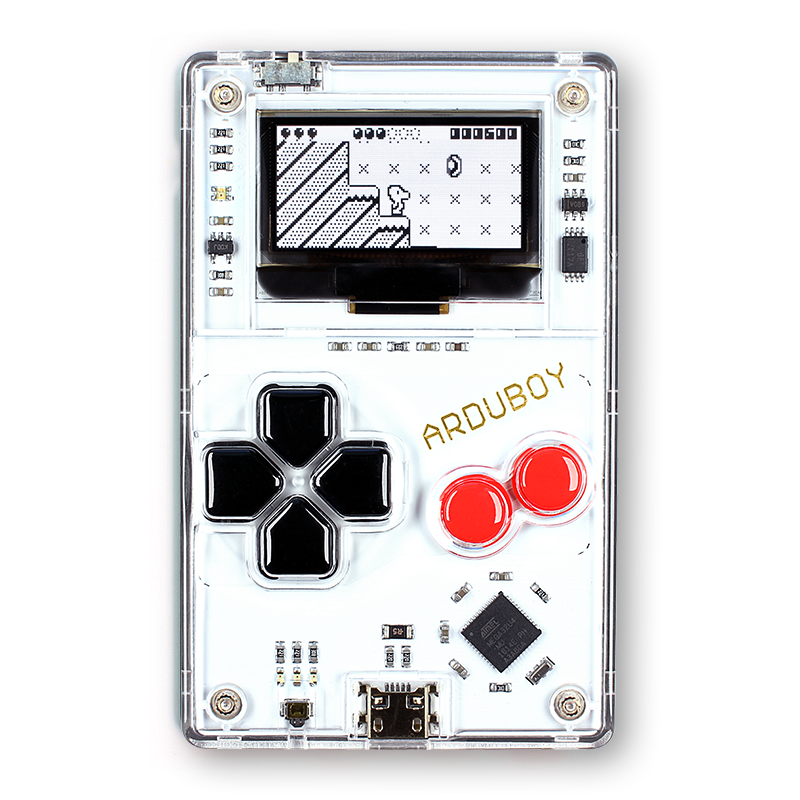
\includegraphics[width=13.4cm]{ArduboyGame.png}
\end{figure}

\section{Preparation}
\label{sec:arduboy-instellingen}
% Arduino Leonardo
% Importeren library

Before we can get started with programming games for the Arduboy, we first have to adjust some settings in the Arduino IDE. For a manual with screenshots you can go to the Arduboy Community~\cite{arduboy:tuto1}.

\subsection{Installing the Arduboy2 library}
The \emph{Arduboy2} library contains a handy interface that ensures that we can easily access all functions of the device. This way we can fully focus on designing and programming the game itself.\\

\noindent
Before we can use this library, it must first be installed in the IDE. You do this as follows:\\

\begin{enumerate}
	\item Click \textbf{Tools} > \textbf{Manage Libraries...}
	\item In the \emph{Library Manager} window search for the library \textbf{Arduboy2}
	\item Choose the latest version then click \textbf{Install}
\end{enumerate}

This way easily install other libraries using this same process if you wish.

\subsection{Installing the Arduboy as an Arduino board}
\index{Board}
\begin{enumerate}
	\item Go to \textbf{File} > \textbf{Preferences}
	\item In the \emph{Preferences} screen, enter the following URL at \textbf{Additional Boards Manager URLs}: \url{https://arduboy.github.io/board-support/package_arduboy_index.json}
	\item Click OK to close the \emph{Preferences} window
	\item Go to \textbf{Tools} > \textbf{Board} > \textbf{Boards Manager...}
	\item Zoek naar \textbf{Arduboy} en klik op \textbf{Installeren}
\end{enumerate}

\subsection{Board Selection}
To let the IDE know that you are programming for the Arduboy, you must select the board in the IDE.

\begin{enumerate}
	\item Go to \textbf{Tools} > \textbf{Board}
	\item Choose \textbf{Arduboy} from the list.
\end{enumerate}


\section{Program Structure}
\index{Program Structure}

\begin{minted}{cpp}
#include <Arduboy2.h>

Arduboy2 arduboy;

void setup() {
  arduboy.begin();
}

void loop() {
  if (arduboy.nextFrame()) {
    arduboy.clear();

    // GAME LOGIC

    arduboy.display();
  }
}
\end{minted}
\noindent
The code fragment above gives a template from which you can start to program an Arduboy game. The Arduboy2 library is included on the first line. A \texttt{Arduboy2} object is then created. This object is used to invoke the functionality of the library. Finally, during \texttt{setup()}, the functionality of the Arduboy is initialized.

\section{The Arduboy2 Library}
\index{Library}
Here we provide an overview of the most important functions in the Arduboy2 library~\cite{arduboy:lib2-doc}. These functions can be used in this way:

\begin{center}
	\texttt{arduboy.function\_name();}
\end{center}
\noindent
Optional parameters for the functions are \emph{italic}.

\subsection{Startup}
These functions are used to properly initialize the Arduboy.

\begin{libf}[begin()]
	Initialize the hardware, display the logo, etc. This function must be called once in the \texttt{setup()} procedure.
\end{libf}

\begin{libf}[initRandomSeed()]
    Choose a random value as \emph{seed} for the random number generator. This method is most effective when it is called after a (semi-) random time.
\end{libf}

\subsection{Display}
These functions relate to the screen of the Arduboy.

\begin{libf}[\textsc{Display}]
	There are the following handy constants for the width and height of the screen. In addition, there are also constants for the colors of the screen.
	\begin{multicols}{2}
		\begin{itemize}
			\item \texttt{WIDTH}
			\item \texttt{HEIGHT}
			\item \texttt{BLACK}
			\item \texttt{WHITE}
		\end{itemize}
	\end{multicols}
\end{libf}

\begin{libf}[clear()]
	Clear the display buffer. The entire screen is set to black.
\end{libf}

\begin{libf}[display()]
	Paint the contents of the display buffer to the screen.
\end{libf}

\begin{libf}[setFrameRate(fps)]
	Sets the desired frame rate.\\ \\
	\textbf{Parameter}
	\begin{itemize}
		\item \texttt{int fps}: desired frame-rate in frames per second
	\end{itemize}
\end{libf}

\begin{libf}[nextFrame()]
	Indicates when it is time to display the next frame.\\ \\
	\textbf{Returns}
	\begin{itemize}
		\item \texttt{bool}: \texttt{true} when it's time for the next frame, otherwise \texttt{false}
	\end{itemize}
\end{libf}

\subsubsection{Drawing}
These functions are used to draw shapes on the screen of the Arduboy.

\begin{libf}[drawPixel(x, y, \emph{color=WHITE})]
	Draws a single pixel in the specified color.\\ \\
	\textbf{Parameters}
	\begin{itemize}
		\item \texttt{int x}: x coordinate of the pixel
		\item \texttt{int y}: y coordinate of the pixel
		\item \texttt{int color} (optional): color $\rightarrow$ \texttt{WHITE} or \texttt{BLACK}
	\end{itemize}
\end{libf}

\begin{libf}[drawCircle(x, y, r, \emph{color=WHITE})]
	Draws a circle.\\ \\
	\textbf{Parameters}
	\begin{itemize}
		\item \texttt{int x}: x coordinate of the center of the circle
		\item \texttt{int y}: y coordinate of the center of the circle
		\item \texttt{int r}: radius of the circle
		\item \texttt{int color} (optional): color $\rightarrow$ \texttt{WHITE} of \texttt{BLACK}
	\end{itemize}
\end{libf}

\begin{libf}[drawRect(x, y, w, h, \emph{color=WHITE})]
	Draws a rectangle.\\ \\
	\textbf{Parameters}
	\begin{itemize}
		\item \texttt{int x}: x coordinate of the top left corner
		\item \texttt{int y}: y coordinate of the top left corner
		\item \texttt{int w}: width
		\item \texttt{int h}: height
		\item \texttt{int color} (optional): color $\rightarrow$ \texttt{WHITE} of \texttt{BLACK}
	\end{itemize}
\end{libf}

\begin{libf}[drawRoundRect(x, y, w, h, r, \emph{color=WHITE})]
	Draws a rectangle with rounded corners.\\ \\
	\textbf{Parameters}
	\begin{itemize}
		\item \texttt{int x}: x coordinate of the top left corner
		\item \texttt{int y}: y coordinate of the top left corner
		\item \texttt{int w}: width
		\item \texttt{int h}: height
		\item \texttt{int r}: radius of the rounding
		\item \texttt{int color} (optional): color $\rightarrow$ \texttt{WHITE} of \texttt{BLACK}
	\end{itemize}
\end{libf}

\begin{libf}[drawTriangle(x0, y0, x1, y1, x2, y2, \emph{color=WHITE})]
	Draws a triangle.\\ \\
	\textbf{Parameters}
	\begin{itemize}
		\item \texttt{int x0, int x1, int x2}: x coordinates of the angles
		\item \texttt{int y0, int y1, int y2}: y coordinates of the angles
		\item \texttt{int color} (optional): color $\rightarrow$ \texttt{WHITE} of \texttt{BLACK}
	\end{itemize}
\end{libf}

\newpage

\begin{libf}[drawLine(x0, y0, x1, y1, \emph{color=WHITE})]
	Draws a line between the specified points.\\ \\
	\textbf{Parameters}
	\begin{itemize}
		\item \texttt{int x0, int x1}: x coordinates of the points
		\item \texttt{int y0, int y1}: y coordinates of the points
		\item \texttt{int color} (optional): color $\rightarrow$ \texttt{WHITE} of \texttt{BLACK}
	\end{itemize}
\end{libf}

\begin{libf}[drawFastVLine(x, y, h, \emph{color=WHITE})]
	Draws a vertical line.\\ \\
	\textbf{Parameters}
	\begin{itemize}
		\item \texttt{int x}: x coordinate of the upper end
		\item \texttt{int y}: y coordinate of the upper end
		\item \texttt{int h}: height
		\item \texttt{int color} (optional): color $\rightarrow$ \texttt{WHITE} of \texttt{BLACK}
	\end{itemize}
\end{libf}

\begin{libf}[drawFastHLine(x, y, w, \emph{color=WHITE})]
	Draws a horizontal line.\\ \\
	\textbf{Parameters}
	\begin{itemize}
		\item \texttt{int x}: x coordinate of the left end
		\item \texttt{int y}: y coordinate of the left end
		\item \texttt{int w}: width
		\item \texttt{int color} (optional): color $\rightarrow$ \texttt{WHITE} of \texttt{BLACK}
	\end{itemize}
\end{libf}

\begin{libf}[fillCircle(x, y, r, \emph{color=WHITE})]
	Draws a filled circle.\\ \\
	\textbf{Parameters}
	\begin{itemize}
		\item \texttt{int x}: x coordinate of the center of the circle
		\item \texttt{int y}: y coordinate of the center of the circle
		\item \texttt{int r}: radius of the circle
		\item \texttt{int color} (optional): color $\rightarrow$ \texttt{WHITE} of \texttt{BLACK}
	\end{itemize}
\end{libf}

\begin{libf}[fillRect(x, y, w, h, \emph{color=WHITE})]
	Draws a filled rectangle.\\ \\
	\textbf{Parameters}
	\begin{itemize}
		\item \texttt{int x}: x coordinate of the top left corner
		\item \texttt{int y}: y coordinate of the top left corner
		\item \texttt{int w}: width
		\item \texttt{int h}: height
		\item \texttt{int color} (optional): color $\rightarrow$ \texttt{WHITE} of \texttt{BLACK}
	\end{itemize}
\end{libf}

\pagebreak

\begin{libf}[fillRoundRect(x, y, w, h, r, \emph{color=WHITE})]
	Teken een opgevulde rechthoek met afgeronde hoeken.\\ \\
	\textbf{Parameters}
	\begin{itemize}
		\item \texttt{int x}: x-coördinaat van de linkerbovenhoek
		\item \texttt{int y}: y-coördinaat van de linkerbovenhoek
		\item \texttt{int w}: breedte
		\item \texttt{int h}: hoogte
		\item \texttt{int r}: straal van de afronding
		\item \texttt{int color} (optioneel): kleur $\rightarrow$ \texttt{WHITE} of \texttt{BLACK}
	\end{itemize}
\end{libf}

\begin{libf}[fillTriangle(x0, y0, x1, y1, x2, y2, \emph{color=WHITE})]
	Teken een opgevulde driehoek.\\ \\
	\textbf{Parameters}
	\begin{itemize}
		\item \texttt{int x0, int x1, int x2}: x-coördinaten van de hoeken
		\item \texttt{int y0, int y1, int y2}: y-coördinaten van de hoeken
		\item \texttt{int color} (optioneel): kleur $\rightarrow$ \texttt{WHITE} of \texttt{BLACK}
	\end{itemize}
\end{libf}

\begin{libf}[fillScreen(\emph{color=WHITE})]
	Vul het scherm op met de opgegeven kleur.\\ \\
	\textbf{Parameters}
	\begin{itemize}
		\item \texttt{int color} (optioneel): kleur $\rightarrow$ \texttt{WHITE} of \texttt{BLACK}
	\end{itemize}
\end{libf}

\subsubsection{Text}
Deze functies worden gebruikt om tekst weer te geven op het scherm van de Arduboy.

\begin{libf}[setCursor(x, y)]
	Stel de locatie van de tekst cursor in.\\ \\
	\textbf{Parameters}
	\begin{itemize}
		\item \texttt{int x}: x-coördinaat
		\item \texttt{int y}: y-coördinaat
	\end{itemize}
\end{libf}

\begin{libf}[setTextSize(s)]
	Stel de grootte van de tekstkarakters in.\\ \\
	\textbf{Parameter}
	\begin{itemize}
		\item \texttt{int s}: tekstgrootte ($\geq 1$)
	\end{itemize}
\end{libf}

\begin{libf}[setTextColor(c)]
	Stel de tekstkleur in.\\ \\
	\textbf{Parameter}
	\begin{itemize}
		\item \texttt{int c}: kleur $\rightarrow$ \texttt{WHITE} of \texttt{BLACK}
	\end{itemize}
\end{libf}

\begin{libf}[setTextBackground(bg)]
	Stel de achtergrondkleur van de tekst in.\\ \\
	\textbf{Parameter}
	\begin{itemize}
		\item \texttt{int bg}: achtergrondkleur $\rightarrow$ \texttt{WHITE} of \texttt{BLACK}
	\end{itemize}
\end{libf}

\begin{libf}[setTextWrap(w)]
	Schakel text wrapping in of uit. Als text wrapping is ingeschakeld wordt de tekst op een nieuwe lijn geplaatst als deze te lang is om op de huidige lijn te passen.\\ \\
	\textbf{Parameter}
	\begin{itemize}
		\item \texttt{bool w}: \texttt{true} om text wrapping in te schakelen, \texttt{false} om uit te schakelen
	\end{itemize}
\end{libf}

% https://mlxxxp.github.io/documents/Arduino/libraries/Arduboy2/Doxygen/html/classPrint.html
\begin{libf}[\href{https://mlxxxp.github.io/documents/Arduino/libraries/Arduboy2/Doxygen/html/classPrint.html}{print(content)}]
	Print de opgegeven content op de plaats van de cursor.\\ \\
	\textbf{Parameter}
	\begin{itemize}
		\item \texttt{content}: tekst die weergegeven moet worden
	\end{itemize}
\end{libf}

\subsection{Buttons}
Met deze functies kan je interacties via de knoppen van de Arduboy programmeren.

\begin{libf}[\textsc{Buttons}]
	Voor de knoppen op de Arduboy zijn de volgende constanten gedefinieerd.
	\begin{multicols}{3}
		\begin{itemize}
			\item \texttt{A\_BUTTON}
			\item \texttt{B\_BUTTON}
			\item \texttt{LEFT\_BUTTON}
			\item \texttt{RIGHT\_BUTTON}
			\item \texttt{UP\_BUTTON}
			\item \texttt{DOWN\_BUTTON}
		\end{itemize}
	\end{multicols}

	Buttons kunnen samengevoegd worden in een mask: \texttt{LEFT\_BUTTON + A\_BUTTON}
\end{libf}

\begin{libf}[pressed(buttons)]
	Test of de opgegeven knoppen ingedrukt worden.\\ \\
	\textbf{Parameters}
	\begin{itemize}
		\item \texttt{int buttons}: een bit-mask die aangeeft welke knoppen getest moeten worden
	\end{itemize}
	\textbf{Returns}
	\begin{itemize}
		\item \texttt{bool}: \texttt{true} als alle knoppen in het opgegeven mask momenteel ingedrukt zijn
	\end{itemize}
\end{libf}

\begin{libf}[notPressed(buttons)]
	Test of de opgegeven knoppen \textbf{niet} ingedrukt worden.\\ \\
	\textbf{Parameters}
	\begin{itemize}
		\item \texttt{int buttons}: een bit-mask die aangeeft welke knoppen getest moeten worden
	\end{itemize}
	\textbf{Returns}
	\begin{itemize}
		\item \texttt{bool}: \texttt{true} als alle knoppen in het opgegeven mask momenteel \textbf{niet} ingedrukt zijn
	\end{itemize}
\end{libf}

\newpage

\subsection{Physics}
Deze functies worden gebruikt om interacties tussen verschillende objecten in je game te berekenen.

\begin{libf}[collide(rect1, rect2)]
	Controleer of twee rechthoeken elkaar snijden.\\ \\
	\textbf{Parameters}
	\begin{itemize}
		\item \texttt{Rect rect1, Rect rect2}: rechthoeken $\rightarrow$ Rect(int x, int y, int width, int height)
	\end{itemize}
	\textbf{Returns}
	\begin{itemize}
		\item \texttt{bool}: \texttt{true} als de opgegeven rechthoeken overlappen
	\end{itemize}
\end{libf}

\begin{libf}[collide(point, rect)]
	Controleer of een punt binnen een rechthoek ligt.\\ \\
	\textbf{Parameters}
	\begin{itemize}
		\item \texttt{Point point}: punt $\rightarrow$ Point(int x, int y)
		\item \texttt{Rect rect}: rechthoek $\rightarrow$ Rect(int x, int y, int width, int height)
	\end{itemize}
\end{libf}

\subsection{LED}
Via deze functies kan je de RGB LED van de Arduboy aansturen.

\begin{libf}[setRGBled(red, green, blue)]
	Stel de helderheid van de verschillende kleuren in de RGB LED in. De RGB LED zijn eigenlijk kleine individuele rode, groene en blauwe LEDs die zeer dicht bij elkaar geplaatst zijn. Door de helderheid van de 3 kleuren aan te passen, kan je verschillende kleuren tonen.
	De helderheid van elke LED kan een waarde aannemen van 0 (volledig uit) tot 255 (volledig aan).\\ \\
	\textbf{Parameters}
	\begin{itemize}
		\item \texttt{int red}: rode component
		\item \texttt{int green}: groene component
		\item \texttt{int blue}: blauwe component
	\end{itemize}
\end{libf}

\begin{libf}[setRGBled(color, val)]
	Stel de helderheid van één van de kleuren in, zonder de andere kleuren aan te passen.\\ \\
	\textbf{Parameters}
	\begin{itemize}
		\item \texttt{int color}: naam van de kleur: \texttt{RED\_LED}, \texttt{GREEN\_LED} of \texttt{BLUE\_LED}
		\item \texttt{int val}: helderheid, waarde tussen 0 en 255
	\end{itemize}
\end{libf}

\newpage
\section{Emulator}
\index{Emulator}
Als je een game aan het programmeren bent, wil je natuurlijk ook kunnen testen of deze werkt op de manier dat jij wil. Daarom bestaan er emulators voor de Arduboy.

\subsection{ProjectABE}
\href{https://felipemanga.github.io/ProjectABE/}{ProjectABE (\texttt{https://felipemanga.github.io/ProjectABE/})} is een online emulator voor de Arduboy.
Je kan je eigen game testen door op het startscherm onder \textbf{My Projects} > \textbf{New Game} te klikken. In het volgende scherm zie je de emulator, zoals in Figuur~\ref{fig:projectabe}.
\begin{wrapfigure}{r}{5.5cm}
	\centering
	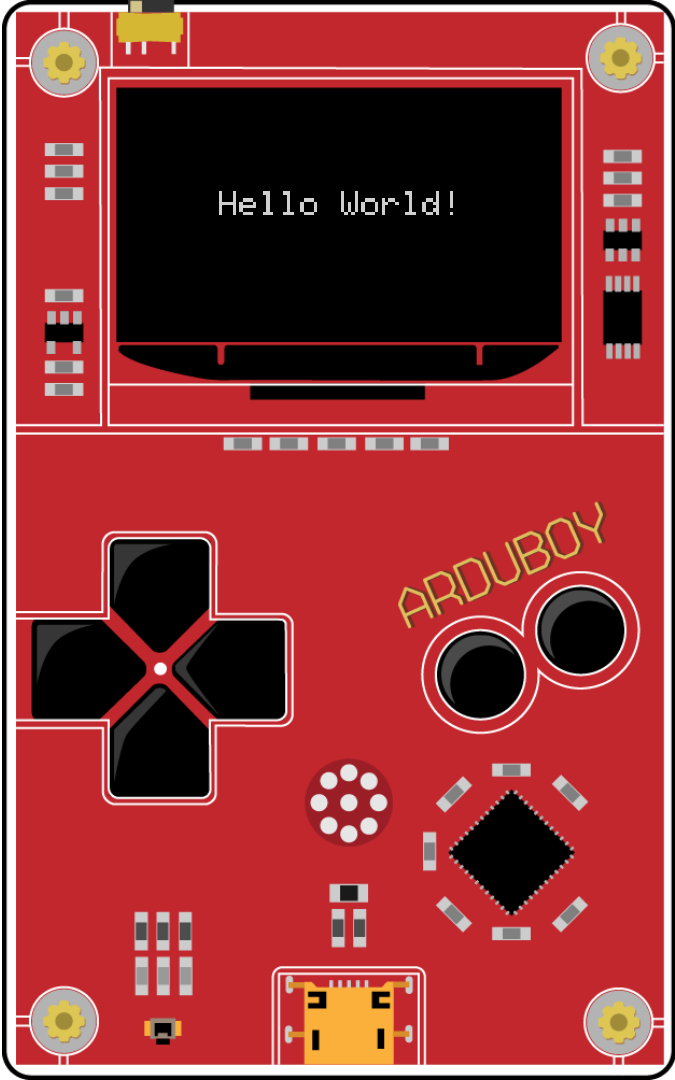
\includegraphics[width=5cm]{assets/ProjectABE}
	\caption{Project ABE}
	\label{fig:projectabe}
\end{wrapfigure}
% export binary
In de Arduino IDE klik je vervolgens op \textbf{Schets} > \textbf{Exporteer gecompileerd Binair bestand}. Hierdoor zal er een bestand met extensie \texttt{.hex} aangemaakt worden in dezelfde map als je code. Dit bestand met extensie \texttt{.hex} sleep je dan naar de emulator. De emulator zal dan meteen jouw code uitvoeren.\\
Je kan de emulator bedienen met het toetsenbord of door te klikken op de knoppen op het scherm.

\section{Programma op Arduboy plaatsen}
Voor je het programma op de Arduboy plaatst, controleer je best of zeker het juiste board\index{Board} geselecteerd is (zie Sectie~\ref{sec:arduboy-instellingen}). Daarna zet je de Arduboy aan en verbind je hem met de computer via de USB-kabel. Vervolgens selecteer je de juiste poort via \textbf{Hulpmiddelen} > \textbf{Poort} en kies dan de optie waar Arduino bij staat.\\
Nu ben je volledig klaar om het programma op de Arduboy te plaatsen. Je moet enkel nog op het pijltje (\textbf{Uploaden}) klikken en even wachten. Als alles goed gaat, staat je programma op de Arduboy.

\vspace{1cm}

\noindent
\emph{Veel gameplezier!}


%----------------------------------------------------------------------------------------
%	BIBLIOGRAPHY
%----------------------------------------------------------------------------------------

\chapterimage{jcw_header.pdf}

\chapter*{Bibliografie}
\addcontentsline{toc}{chapter}{\textcolor{ocre}{Bibliografie}} % Add a Bibliography heading to the table of contents

\printbibliography[heading=bibempty]

%----------------------------------------------------------------------------------------
%	INDEX
%----------------------------------------------------------------------------------------

\cleardoublepage % Make sure the index starts on an odd (right side) page
\phantomsection
\setlength{\columnsep}{0.75cm} % Space between the 2 columns of the index
\addcontentsline{toc}{chapter}{\textcolor{ocre}{Index}} % Add an Index heading to the table of contents
\printindex % Output the index

%----------------------------------------------------------------------------------------

\end{document}
